\subsection{Helicopter structure}
At its core, Ingenuity features a fuselage designed for minimal weight and maximum strength, a sturdy framework for housing critical components such as the avionics, power system, and rotor assembly.

The most prominent feature is its coaxial rotor system, comprising two horizontally-overlapping counter-rotating (to mitigate reaction torque effects) blades, ensuring stability and precise maneuverability during flight. Attached to the rotor system is a central mast, which extends upward from the fuselage.

\begin{figure}[H]
    \centering
    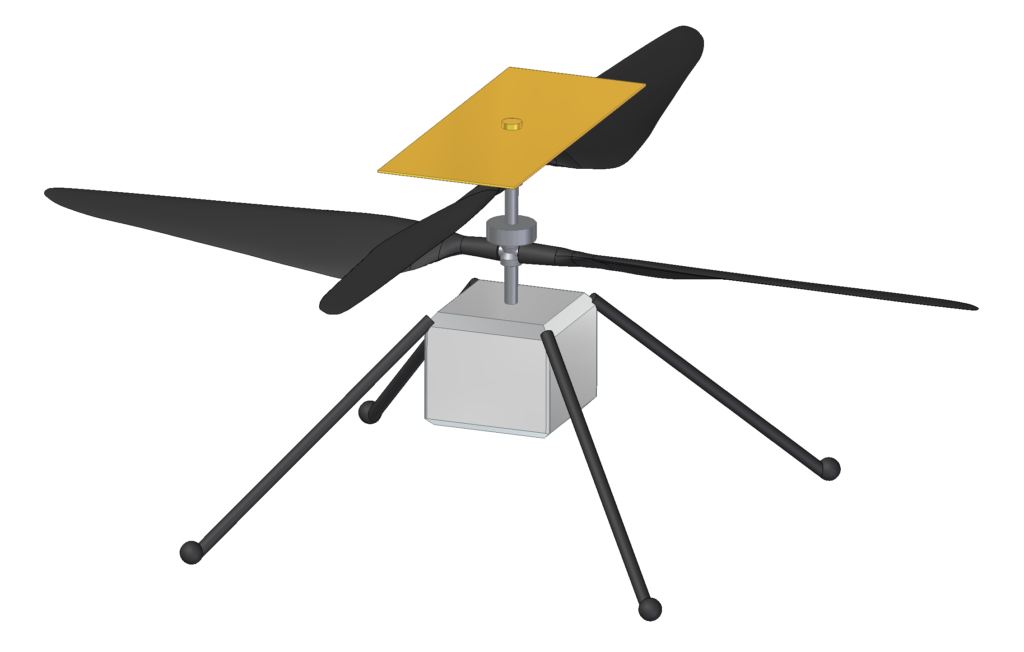
\includegraphics[width=0.7\columnwidth]{figures/ingenuity_render.png}
    \caption{3D render of the Ingenuity Mars Helicopter.}
    \label{fig:ingenuity_render}
\end{figure}

Complementing these is a suite of sensors, cameras, and communication equipment strategically integrated throughout Ingenuity's structure. These instruments enable it to navigate autonomously according to the instructions coming from the base of operation on Earth and capture imagery of the Martian surface.

The main parameters of the helicopter structure model are summarized in Table \ref{tab:ingenuity_parameters}.

\begin{table}[H]
    \centering
    \begin{tabular}{|c|c|c|}
        \hline
        \textbf{Parameter} & \textbf{Symbol} & \textbf{Value} \\
        \hline
        \hline
        Mass & $m$ & \SI{1.8}{\kilogram} \\
        \hline
        Rotor diameter & $2\,r$ & \SI{1.2}{\meter} \\
        \hline
        Blade chord & $c$ & \SI{0.24}{\meter} \\
        \hline
        \begin{tabular}{@{}c@{}}COM - upper\\rotor distance\end{tabular} & $d_{cm, u}$ & \SI{0.10}{\meter} \\
        \hline
        \begin{tabular}{@{}c@{}}COM - lower\\rotor distance\end{tabular} & $d_{cm, l}$ & \SI{0.05}{\meter} \\
        \hline
        Inertia & $I$ & \begin{tabular}{@{}c@{}}$diag(0.210, 0.288, $\\$0.278)$\,\SI{}{\kilogram\square\meter}\end{tabular} \\
        \hline
    \end{tabular}
    \caption{Structural parameters of the Ingenuity model.}
    \label{tab:ingenuity_parameters}
\end{table}
